% Figure 1: profile_1_success
\begin{figure}[t]
  \centering
  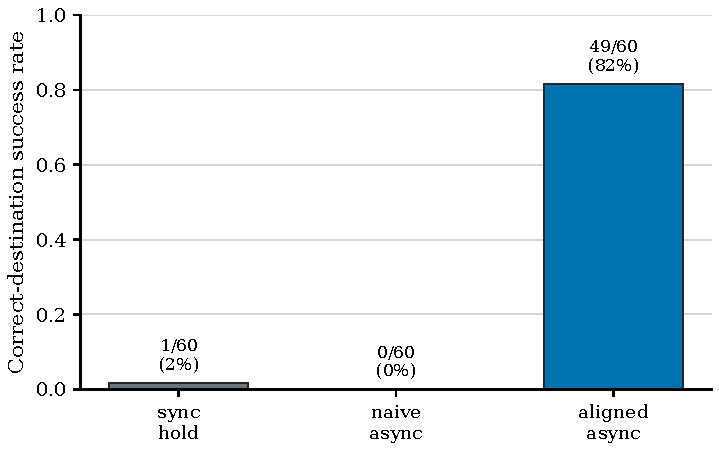
\includegraphics[width=0.48\textwidth]{profile_1_success.pdf}
  \caption{Correct-destination success under the frozen fixed-latency Profile 1. Labels report raw successes and exact paired denominators.}
  \label{fig:m8-profile-1-success}
\end{figure}

% Figure 2: profile_1_recovery_latency
\begin{figure}[t]
  \centering
  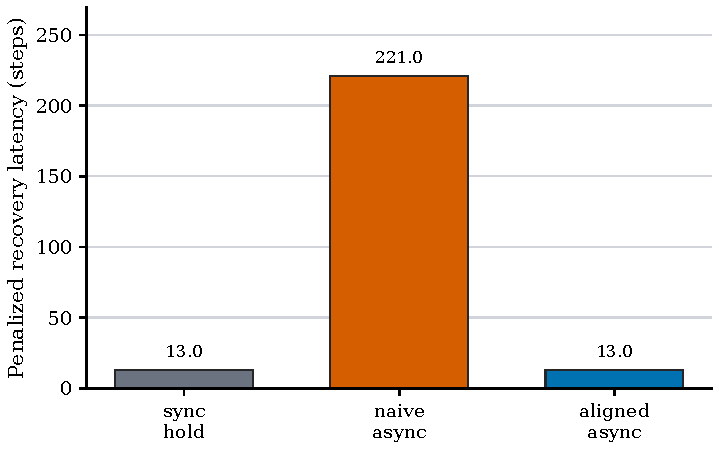
\includegraphics[width=0.48\textwidth]{profile_1_recovery_latency.pdf}
  \caption{Median penalized control-step latency from the destination switch to the first executed post-switch-generation command under Profile 1; lower is better.}
  \label{fig:m8-profile-1-recovery-latency}
\end{figure}

% Figure 3: profile_1_obsolete_commands
\begin{figure}[t]
  \centering
  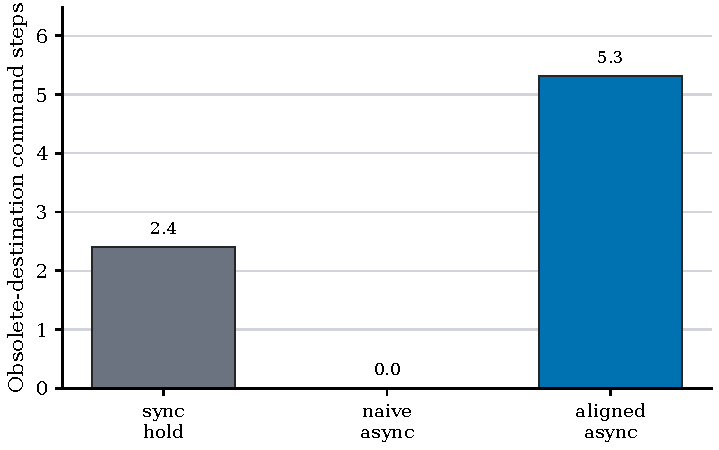
\includegraphics[width=0.48\textwidth]{profile_1_obsolete_commands.pdf}
  \caption{Mean post-switch control steps whose Cartesian commands are geometrically closer to the obsolete destination than the active destination under Profile 1; lower is better.}
  \label{fig:m8-profile-1-obsolete-commands}
\end{figure}
